% Appendix 1

\chapter{Results from Python computation} % Main appendix title

\label{Appendix1} % For referencing this appendix elsewhere, use \ref{Appendix1}

%%%%%%%%%%%%%%%%%%%%%%%%%%%%%%%%%%%%%%%%%%%%%%%%%
%Section 1
%%%%%%%%%%%%%%%%%%%%%%%%%%%%%%%%%%%%%%%%%%%%%%%%%

\section{Results in mode I for $\alpha=0 ^\circ$}

\subsection{e0e1}

\begin{figure}[H]
	\centering
	\begin{subfigure}{0.48\linewidth}
		\centering
		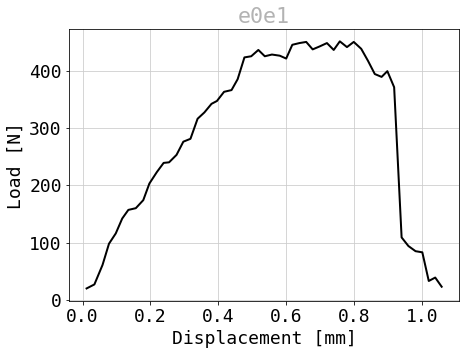
\includegraphics[width=\textwidth]{P_e0e1}
		\decoRule
		\caption{P-Delta curve, for e0e1 specimen.}
		\label{fig:P_e0e1}
	\end{subfigure}
	\hfill 
	\begin{subfigure}{0.48\linewidth}
		\centering
		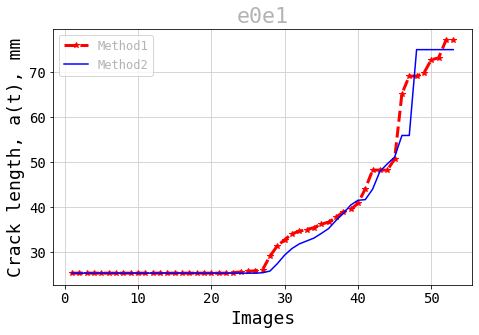
\includegraphics[width=\textwidth]{a_e0e1}
		\decoRule
		\caption{Crack length depending on time, for e0e1 specimen.}
		\label{fig:a_e0e1}
	\end{subfigure}
	\hfill\\
	\begin{subfigure}{0.48\linewidth}
		\centering
		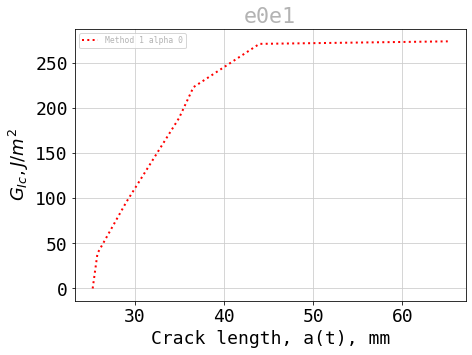
\includegraphics[width=\textwidth]{Gmet1_e0e1}
		\decoRule
		\caption{Energy release rate depending on the crack length propagation method 1, for e0e1 specimen.}
		\label{fig:Gmet1_e0e1}
	\end{subfigure}
	\hfill
	\begin{subfigure}{0.48\linewidth}
		\centering
		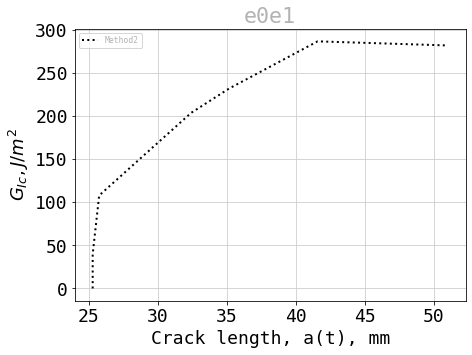
\includegraphics[width=\textwidth]{Gmet2_e0e1}
		\decoRule
		\caption{Energy release rate depending on the crack length propagation method 2, for e0e1 specimen.}
		\label{fig:Gmet2_e0e1}
	\end{subfigure}
	\caption{Mechanical fracture characteristics of specimen e0e1}
	\label{e0e1}
\end{figure}

\subsection{e0e2}

\begin{figure}[H]
	\centering
	\begin{subfigure}{0.48\linewidth}
		\centering
		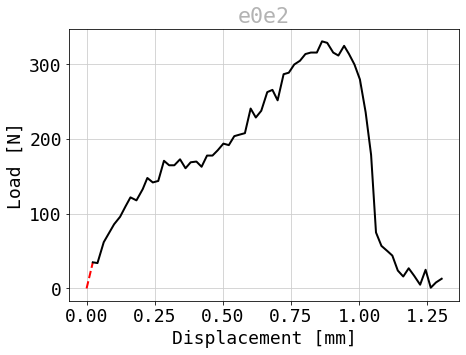
\includegraphics[width=\textwidth]{P_e0e2}
		\decoRule
		\caption{P-Delta curve, for e0e2 specimen.}
		\label{fig:P_e0e2}
	\end{subfigure}
	\hfill 
	\begin{subfigure}{0.48\linewidth}
		\centering
		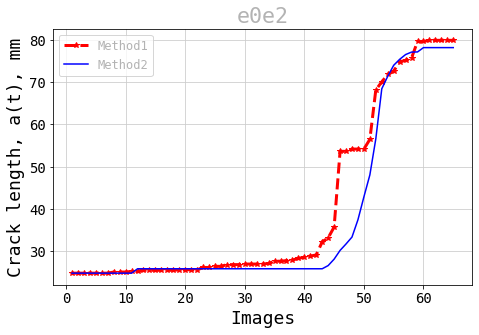
\includegraphics[width=\textwidth]{a_e0e2}
		\decoRule
		\caption{Crack length depending on time, for e0e2 specimen.}
		\label{fig:a_e0e2}
	\end{subfigure}
	\hfill\\
	\begin{subfigure}{0.48\linewidth}
		\centering
		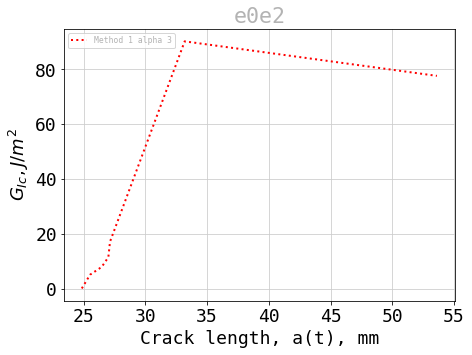
\includegraphics[width=\textwidth]{Gmet1_e0e2}
		\decoRule
		\caption{Energy release rate depending on the crack length propagation method 1, for e0e2 specimen.}
		\label{fig:Gmet1_e0e2}
	\end{subfigure}
	\hfill
	\begin{subfigure}{0.48\linewidth}
		\centering
		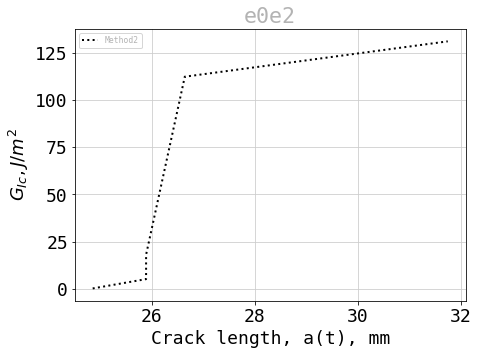
\includegraphics[width=\textwidth]{Gmet2_e0e2}
		\decoRule
		\caption{Energy release rate depending on the crack length propagation method 2, for e0e2 specimen.}
		\label{fig:Gmet2_e0e2}
	\end{subfigure}
	\caption{Mechanical fracture characteristics of specimen e0e2}
	\label{e0e2}
\end{figure}

\subsection{e0e3}

\begin{figure}[H]
	\centering
	\begin{subfigure}{0.48\linewidth}
		\centering
		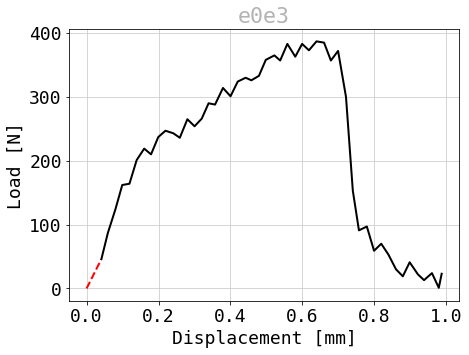
\includegraphics[width=\textwidth]{P_e0e3}
		\decoRule
		\caption{P-Delta curve, for e0e3 specimen.}
		\label{fig:P_e0e3}
	\end{subfigure}
	\hfill 
	\begin{subfigure}{0.48\linewidth}
		\centering
		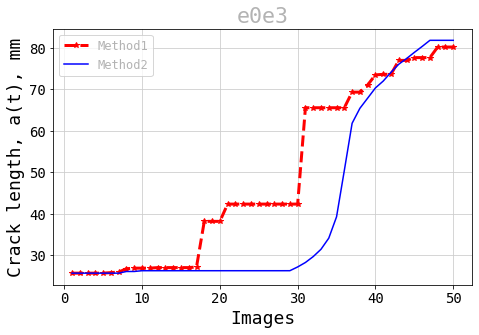
\includegraphics[width=\textwidth]{a_e0e3}
		\decoRule
		\caption{Crack length depending on time, for e0e3 specimen.}
		\label{fig:a_e0e3}
	\end{subfigure}
	\hfill\\
	\begin{subfigure}{0.48\linewidth}
		\centering
		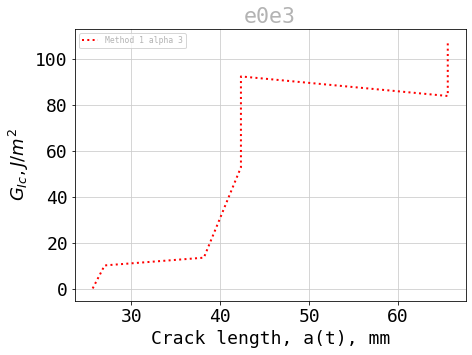
\includegraphics[width=\textwidth]{Gmet1_e0e3}
		\decoRule
		\caption{Energy release rate depending on the crack length propagation method 1, for e0e3 specimen.}
		\label{fig:Gmet1_e0e3}
	\end{subfigure}
	\hfill
	\begin{subfigure}{0.48\linewidth}
		\centering
		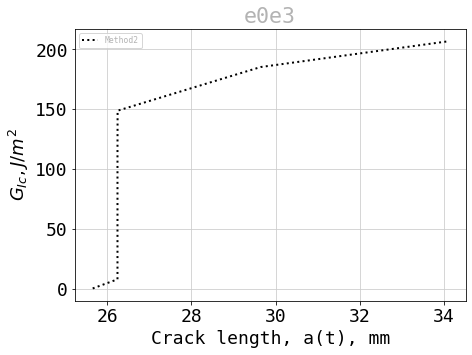
\includegraphics[width=\textwidth]{Gmet2_e0e3}
		\decoRule
		\caption{Energy release rate depending on the crack length propagation method 2, for e0e3 specimen.}
		\label{fig:Gmet2_e0e3}
	\end{subfigure}
	\caption{Mechanical fracture characteristics of specimen e0e3}
	\label{e0e3}
\end{figure}

\subsection{e0e5}

\begin{figure}[H]
	\centering
	\begin{subfigure}{0.48\linewidth}
		\centering
		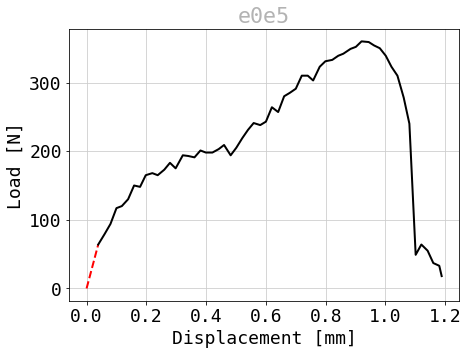
\includegraphics[width=\textwidth]{P_e0e5}
		\decoRule
		\caption{P-Delta curve, for e0e5 specimen.}
		\label{fig:P_e0e5}
	\end{subfigure}
	\hfill 
	\begin{subfigure}{0.48\linewidth}
		\centering
		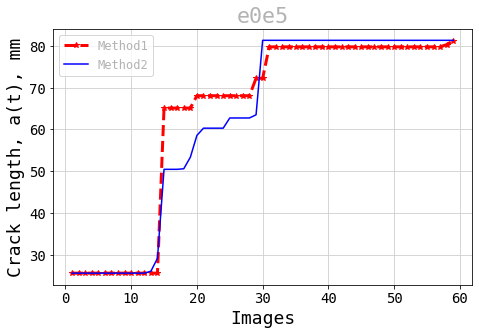
\includegraphics[width=\textwidth]{a_e0e5}
		\decoRule
		\caption{Crack length depending on time, for e0e5 specimen.}
		\label{fig:a_e0e5}
	\end{subfigure}
	\hfill\\
	\begin{subfigure}{0.48\linewidth}
		\centering
		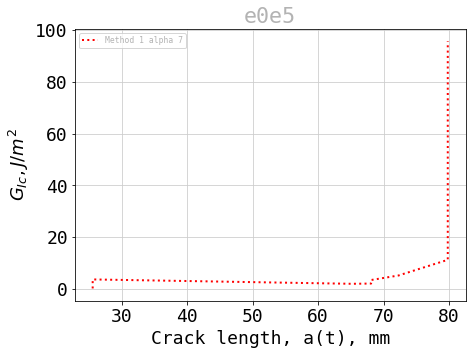
\includegraphics[width=\textwidth]{Gmet1_e0e5}
		\decoRule
		\caption{Energy release rate depending on the crack length propagation method 1, for e15e4 specimen.}
		\label{fig:Gmet1_e0e5}
	\end{subfigure}
	\hfill
	\begin{subfigure}{0.48\linewidth}
		\centering
		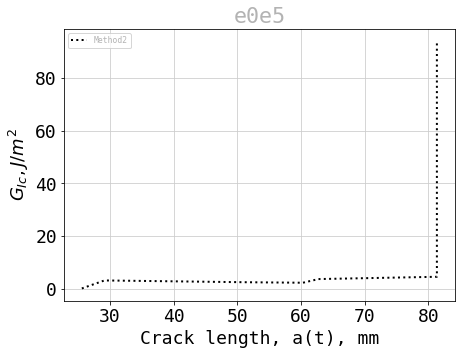
\includegraphics[width=\textwidth]{Gmet2_e0e5}
		\decoRule
		\caption{Energy release rate depending on the crack length propagation method 2, for e0e5 specimen.}
		\label{fig:Gmet2_e0e5}
	\end{subfigure}
	\caption{Mechanical fracture characteristics of specimen e0e5}
	\label{e0e5}
\end{figure}

\subsection{e0e6}

\begin{figure}[H]
	\centering
	\begin{subfigure}{0.48\linewidth}
		\centering
		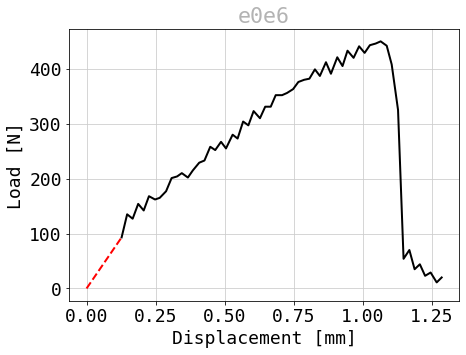
\includegraphics[width=\textwidth]{P_e0e6}
		\decoRule
		\caption{P-Delta curve, for e0e6 specimen.}
		\label{fig:P_e0e6}
	\end{subfigure}
	\hfill 
	\begin{subfigure}{0.48\linewidth}
		\centering
		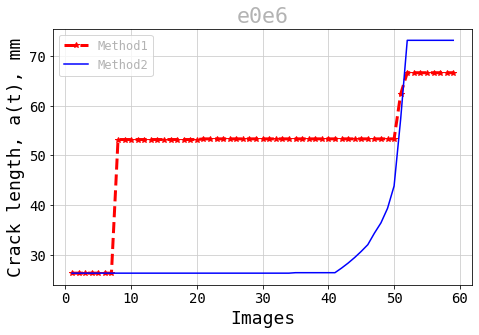
\includegraphics[width=\textwidth]{a_e0e6}
		\decoRule
		\caption{Crack length depending on time, for e0e6 specimen.}
		\label{fig:a_e0e6}
	\end{subfigure}
	\hfill\\
	\begin{subfigure}{0.48\linewidth}
		\centering
		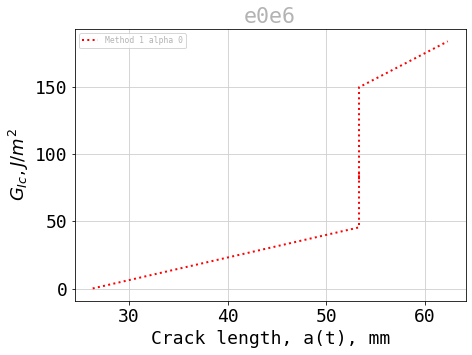
\includegraphics[width=\textwidth]{Gmet1_e0e6}
		\decoRule
		\caption{Energy release rate depending on the crack length propagation method 1, for e0e6 specimen.}
		\label{fig:Gmet1_e0e6}
	\end{subfigure}
	\hfill 
	\begin{subfigure}{0.48\linewidth}
		\centering
		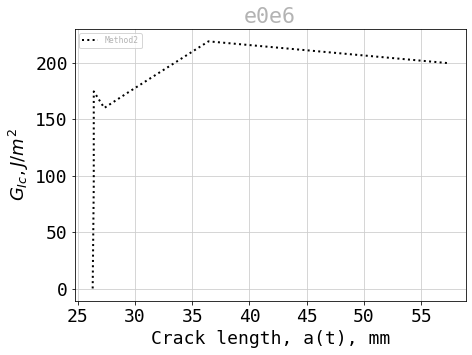
\includegraphics[width=\textwidth]{Gmet2_e0e6}
		\decoRule
		\caption{Energy release rate depending on the crack length propagation method 2, for e0e6 specimen.}
		\label{fig:Gmet2_e0e6}
	\end{subfigure}
	\caption{Mechanical fracture characteristics of specimen e0e6}
	\label{e0e6}
\end{figure}



\section{Results in mixed mode for $\alpha=15 ^\circ$}

\subsection{e15e1}

\begin{figure}[H]
	\centering
\begin{subfigure}{0.48\linewidth}
	\centering
	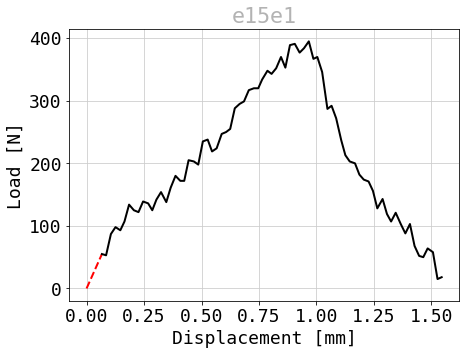
\includegraphics[width=\textwidth]{P_e15e1}
	\decoRule
	\caption{P-Delta curve, for e15e1 specimen.}
	\label{fig:P_e15e1}
\end{subfigure}
\hfill \\
\begin{subfigure}{0.48\linewidth}
	\centering
	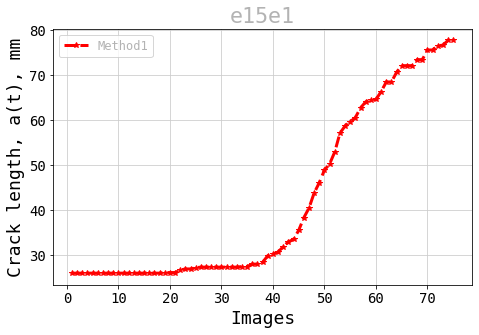
\includegraphics[width=\textwidth]{a_e15e1}
	\decoRule
	\caption{Crack length depending on time, for e15e1 specimen.}
	\label{fig:a_e15e1}
\end{subfigure}
\hfill\\
\begin{subfigure}{0.48\linewidth}
	\centering
	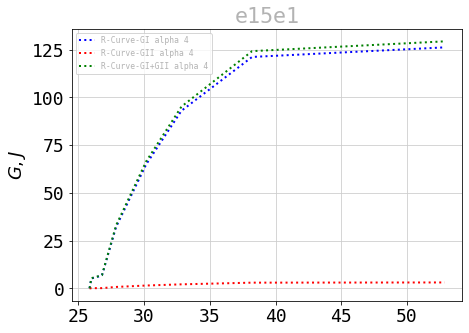
\includegraphics[width=\textwidth]{G_e15e1}
	\decoRule
	\caption{Energy release rate depending on the crack length propagation, for e15e1 specimen.}
	\label{fig:G_e15e1}
\end{subfigure}
\caption{Mechanical fracture characteristics of specimen e15e1}
\label{e15e1}
\end{figure}

\subsection{e15e2}

\begin{figure}[H]
	\centering
	\begin{subfigure}{0.48\linewidth}
		\centering
		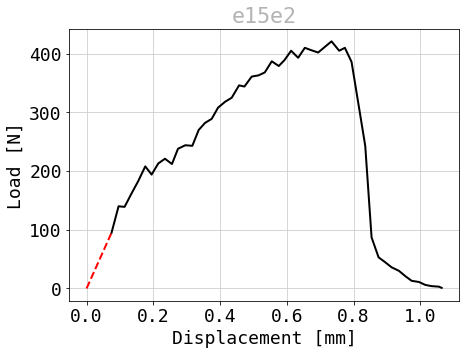
\includegraphics[width=\textwidth]{P_e15e2}
		\decoRule
		\caption{P-Delta curve, for e15e2 specimen.}
		\label{fig:P_e15e2}
	\end{subfigure}
	\hfill \\
	\begin{subfigure}{0.48\linewidth}
		\centering
		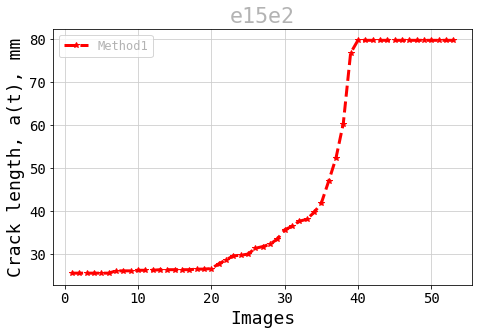
\includegraphics[width=\textwidth]{a_e15e2}
		\decoRule
		\caption{Crack length depending on time, for e15e2 specimen.}
		\label{fig:a_e15e2}
	\end{subfigure}
	\hfill\\
	\begin{subfigure}{0.48\linewidth}
		\centering
		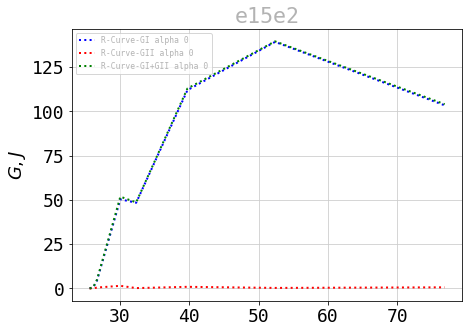
\includegraphics[width=\textwidth]{G_e15e2}
		\decoRule
		\caption{Energy release rate depending on the crack length propagation, for e15e2 specimen.}
		\label{fig:G_e15e2}
	\end{subfigure}
	\caption{Mechanical fracture characteristics of specimen e15e2}
	\label{e15e2}
\end{figure}

\subsection{e15e3}

\begin{figure}[H]
	\centering
	\begin{subfigure}{0.48\linewidth}
		\centering
		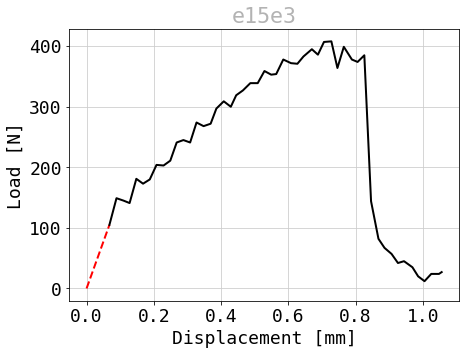
\includegraphics[width=\textwidth]{P_e15e3}
		\decoRule
		\caption{P-Delta curve, for e15e3 specimen.}
		\label{fig:P_e15e3}
	\end{subfigure}
	\hfill \\
	\begin{subfigure}{0.48\linewidth}
		\centering
		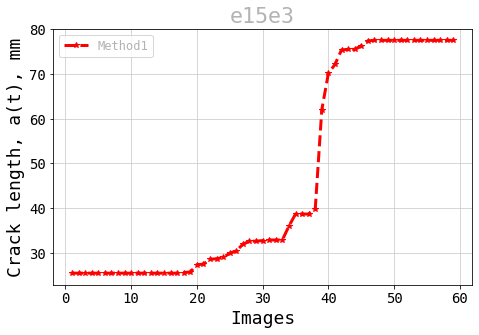
\includegraphics[width=\textwidth]{a_e15e3}
		\decoRule
		\caption{Crack length depending on time, for e15e3 specimen.}
		\label{fig:a_e15e3}
	\end{subfigure}
	\hfill\\
	\begin{subfigure}{0.48\linewidth}
		\centering
		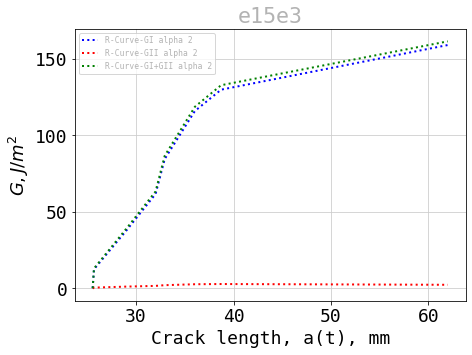
\includegraphics[width=\textwidth]{G_e15e3}
		\decoRule
		\caption{Energy release rate depending on the crack length propagation, for e15e3 specimen.}
		\label{fig:G_e15e3}
	\end{subfigure}
	\caption{Mechanical fracture characteristics of specimen e15e3}
	\label{e15e3}
\end{figure}

\subsection{e15e4}

\begin{figure}[H]
	\centering
	\begin{subfigure}{0.48\linewidth}
		\centering
		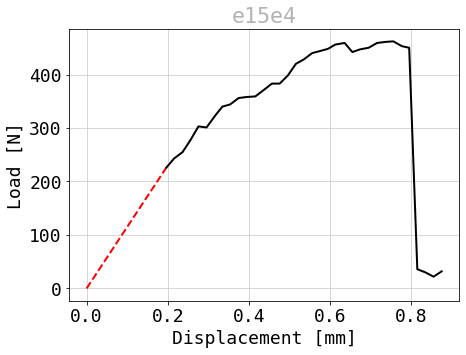
\includegraphics[width=\textwidth]{P_e15e4}
		\decoRule
		\caption{P-Delta curve, for e15e4 specimen.}
		\label{fig:P_e15e3}
	\end{subfigure}
	\hfill \\
	\begin{subfigure}{0.48\linewidth}
		\centering
		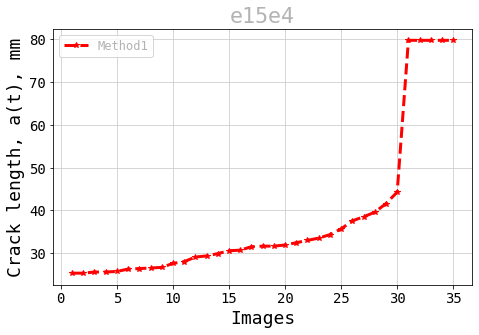
\includegraphics[width=\textwidth]{a_e15e4}
		\decoRule
		\caption{Crack length depending on time, for e15e4 specimen.}
		\label{fig:a_e15e4}
	\end{subfigure}
	\hfill\\
	\begin{subfigure}{0.48\linewidth}
		\centering
		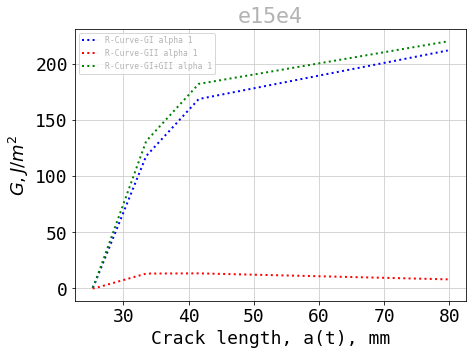
\includegraphics[width=\textwidth]{G_e15e4}
		\decoRule
		\caption{Energy release rate depending on the crack length propagation, for e15e4 specimen.}
		\label{fig:G_e15e4}
	\end{subfigure}
	\caption{Mechanical fracture characteristics of specimen e15e4}
	\label{e15e4}
\end{figure}

\subsection{e15e5}

\begin{figure}[H]
	\centering
	\begin{subfigure}{0.48\linewidth}
		\centering
		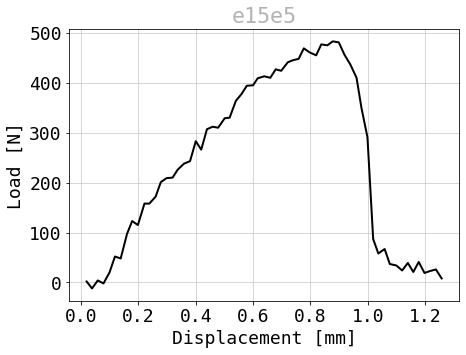
\includegraphics[width=\textwidth]{P_e15e5}
		\decoRule
		\caption{P-Delta curve, for e15e5 specimen.}
		\label{fig:P_e15e5}
	\end{subfigure}
	\hfill \\
	\begin{subfigure}{0.48\linewidth}
		\centering
		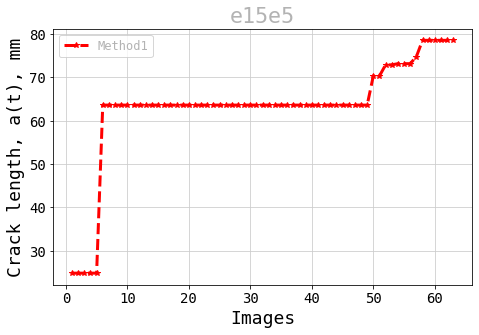
\includegraphics[width=\textwidth]{a_e15e5}
		\decoRule
		\caption{Crack length depending on time, for e15e5 specimen.}
		\label{fig:a_e15e5}
	\end{subfigure}
	\hfill\\
	\begin{subfigure}{0.48\linewidth}
		\centering
		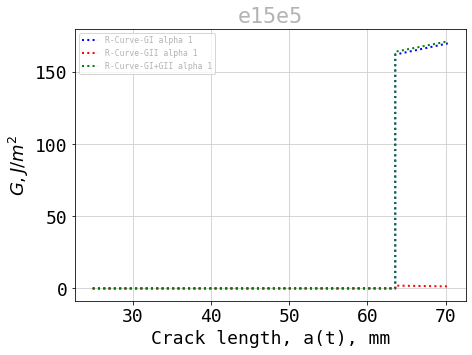
\includegraphics[width=\textwidth]{G_e15e5}
		\decoRule
		\caption{Energy release rate depending on the crack length propagation, for e15e5 specimen.}
		\label{fig:G_e15e5}
	\end{subfigure}
	\caption{Mechanical fracture characteristics of specimen e15e5}
	\label{e15e5}
\end{figure}



\section{Results in mixed mode for $\alpha=30 ^\circ$}

\subsection{e30e2}

\begin{figure}[H]
	\centering
	\begin{subfigure}{0.48\linewidth}
		\centering
		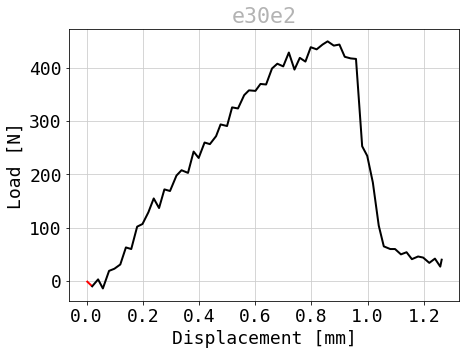
\includegraphics[width=\textwidth]{P_e30e2}
		\decoRule
		\caption{P-Delta curve, for e15e1 specimen.}
		\label{fig:P_e30e2}
	\end{subfigure}
	\hfill \\
	\begin{subfigure}{0.48\linewidth}
		\centering
		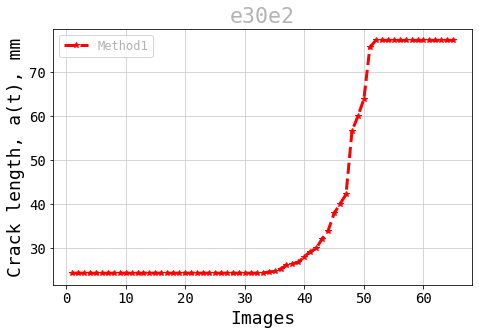
\includegraphics[width=\textwidth]{a_e30e2}
		\decoRule
		\caption{Crack length depending on time, for e15e1 specimen.}
		\label{fig:a_e30e2}
	\end{subfigure}
	\hfill\\
	\begin{subfigure}{0.48\linewidth}
		\centering
		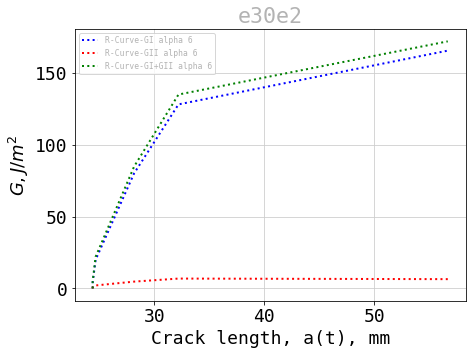
\includegraphics[width=\textwidth]{G_e30e2}
		\decoRule
		\caption{Energy release rate depending on the crack length propagation, for e15e1 specimen.}
		\label{fig:G_e30e2}
	\end{subfigure}
	\caption{Mechanical fracture characteristics of specimen e30e2}
	\label{e30e2}
\end{figure}

\subsection{e30e3}

\begin{figure}[H]
	\centering
	\begin{subfigure}{0.48\linewidth}
		\centering
		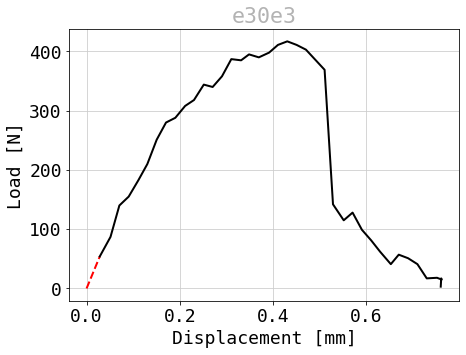
\includegraphics[width=\textwidth]{P_e30e3}
		\decoRule
		\caption{P-Delta curve, for e30e3 specimen.}
		\label{fig:P_e30e3}
	\end{subfigure}
	\hfill \\
	\begin{subfigure}{0.48\linewidth}
		\centering
		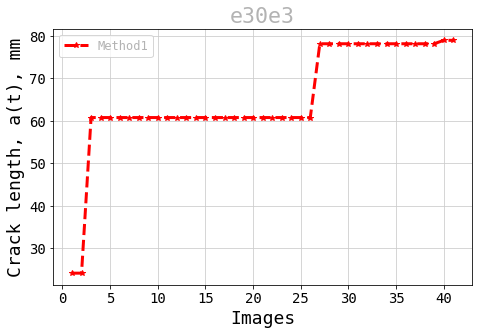
\includegraphics[width=\textwidth]{a_e30e3}
		\decoRule
		\caption{Crack length depending on time, for e30e3 specimen.}
		\label{fig:a_e30e3}
	\end{subfigure}
	\hfill\\
	\begin{subfigure}{0.48\linewidth}
		\centering
		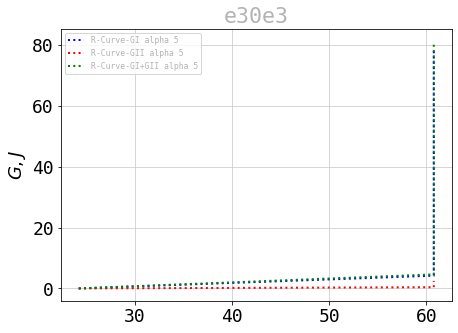
\includegraphics[width=\textwidth]{G_e30e3}
		\decoRule
		\caption{Energy release rate depending on the crack length propagation, for e30e3 specimen.}
		\label{fig:G_e30e3}
	\end{subfigure}
	\caption{Mechanical fracture characteristics of specimen e30e3}
	\label{e30e3}
\end{figure}

\subsection{e30e5}

\begin{figure}[H]
	\centering
	\begin{subfigure}{0.48\linewidth}
		\centering
		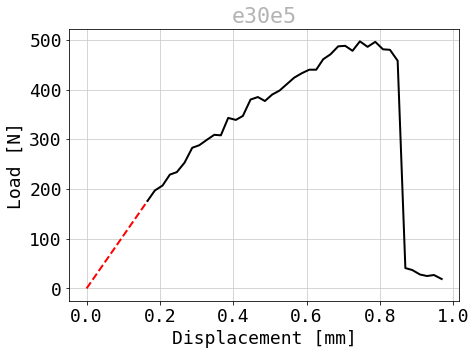
\includegraphics[width=\textwidth]{P_e30e5}
		\decoRule
		\caption{P-Delta curve, for e30e5 specimen.}
		\label{fig:P_e30e5}
	\end{subfigure}
	\hfill \\
	\begin{subfigure}{0.48\linewidth}
		\centering
		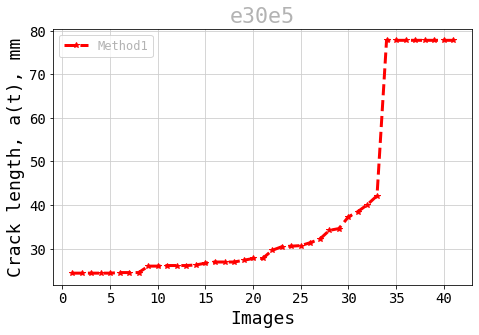
\includegraphics[width=\textwidth]{a_e30e5}
		\decoRule
		\caption{Crack length depending on time, for e30e5 specimen.}
		\label{fig:a_e30e5}
	\end{subfigure}
	\hfill\\
	\begin{subfigure}{0.48\linewidth}
		\centering
		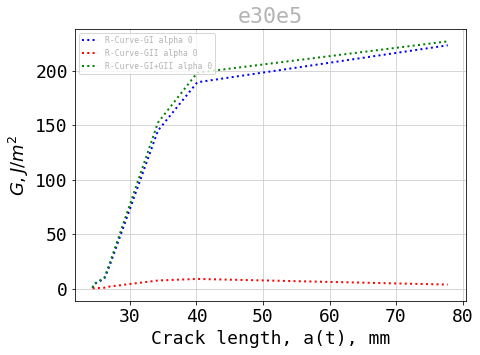
\includegraphics[width=\textwidth]{G_e30e5}
		\decoRule
		\caption{Energy release rate depending on the crack length propagation, for e30e5 specimen.}
		\label{fig:G_e30e5}
	\end{subfigure}
	\caption{Mechanical fracture characteristics of specimen e30e5}
	\label{e30e5}
\end{figure}

\subsection{e30e7}

\begin{figure}[H]
	\centering
	\begin{subfigure}{0.48\linewidth}
		\centering
		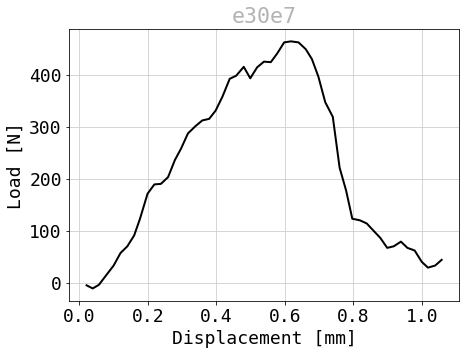
\includegraphics[width=\textwidth]{P_e30e7}
		\decoRule
		\caption{P-Delta curve, for e30e7 specimen.}
		\label{fig:P_e30e7}
	\end{subfigure}
	\hfill \\
	\begin{subfigure}{0.48\linewidth}
		\centering
		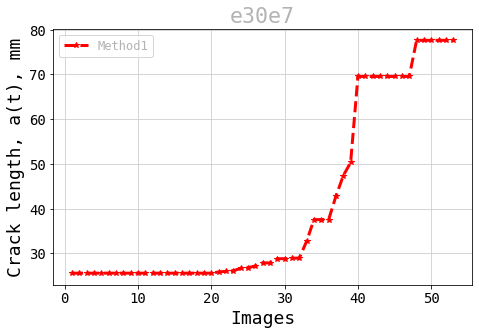
\includegraphics[width=\textwidth]{a_e30e7}
		\decoRule
		\caption{Crack length depending on time, for e30e7 specimen.}
		\label{fig:a_e30e7}
	\end{subfigure}
	\hfill\\
	\begin{subfigure}{0.48\linewidth}
		\centering
		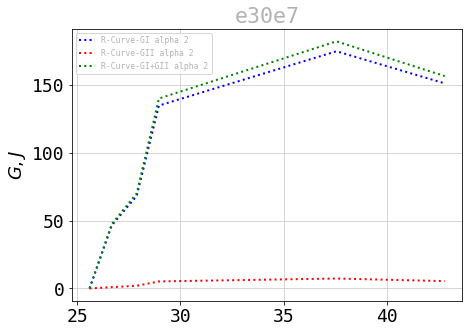
\includegraphics[width=\textwidth]{G_e30e7}
		\decoRule
		\caption{Energy release rate depending on the crack length propagation, for e30e7 specimen.}
		\label{fig:G_e30e7}
	\end{subfigure}
	\caption{Mechanical fracture characteristics of specimen e30e7}
	\label{e30e7}
\end{figure}





